\documentclass[12pt, a4paper]{article}

% --- Paquetes básicos ---
\usepackage[utf8]{inputenc}
\usepackage[spanish]{babel}
\usepackage[margin=2.5cm]{geometry}
\usepackage{graphicx}
\usepackage{float}
\usepackage{amsmath, amssymb}
\usepackage{fancyhdr}

% --- Configuración del Título ---
\title{Bloque 2: Simulación de Carga de Trabajo y Monitorización}
\author{Juan Reche Aguilar}
\date{\today}

% --- Configuración de Encabezados ---
\pagestyle{fancy}
\fancyhf{}
\rhead{Ingeniería de Servidores}
\lhead{Juan Reche Aguilar}
\cfoot{\thepage}

\begin{document}

\maketitle

\tableofcontents
\newpage

\section{Ejercicio 2.1.1.  Ejecutar un Benchmark}

\begin{figure}[H]
    \centering

    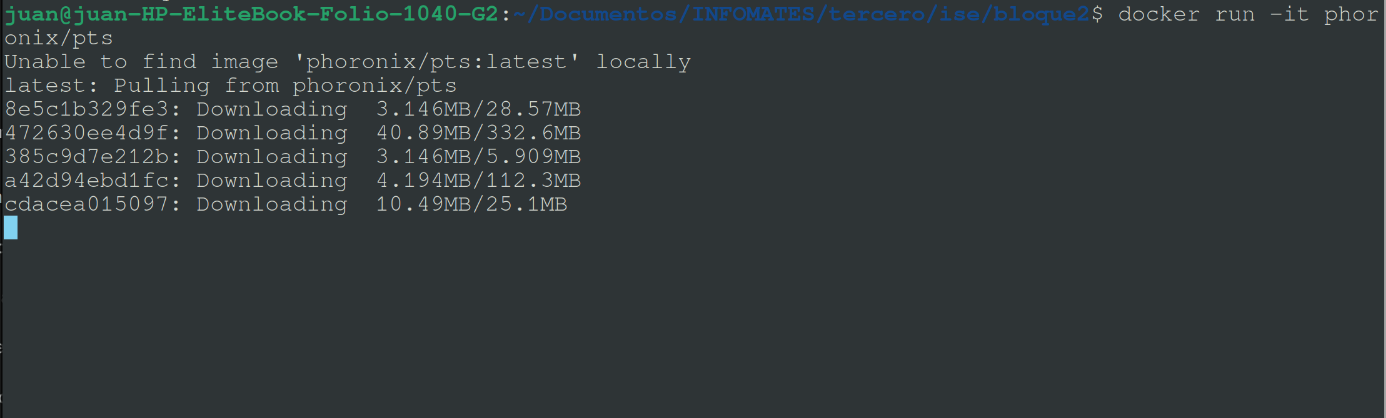
\includegraphics[width=1\textwidth]{../../capturas2/seccion1/run_inicial.png}

    \caption{comando para iniciar phoronix.}

\end{figure}
\begin{figure}[H]
    \centering

    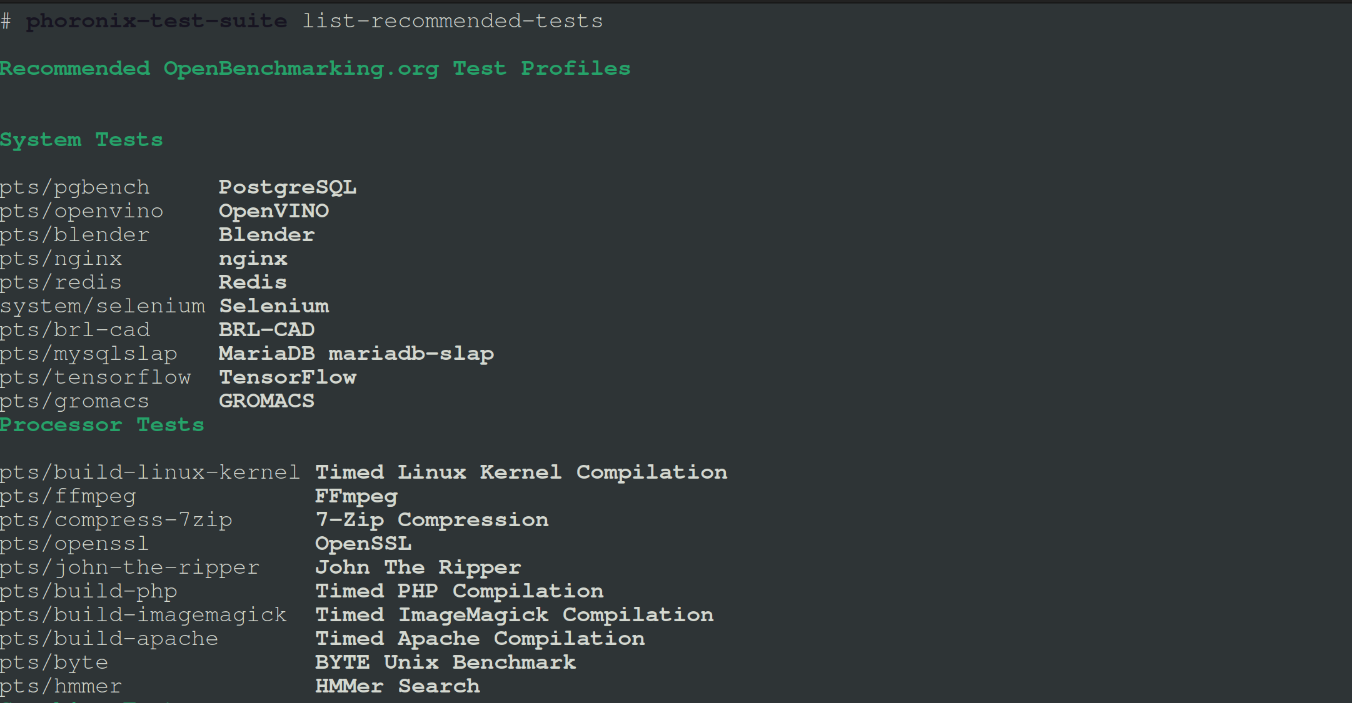
\includegraphics[width=1\textwidth]{../../capturas2/seccion1/test_recomendados.png}

    \caption{Mostramos varios test recomendados.}

\end{figure}
\begin{figure}[H]
    \centering

    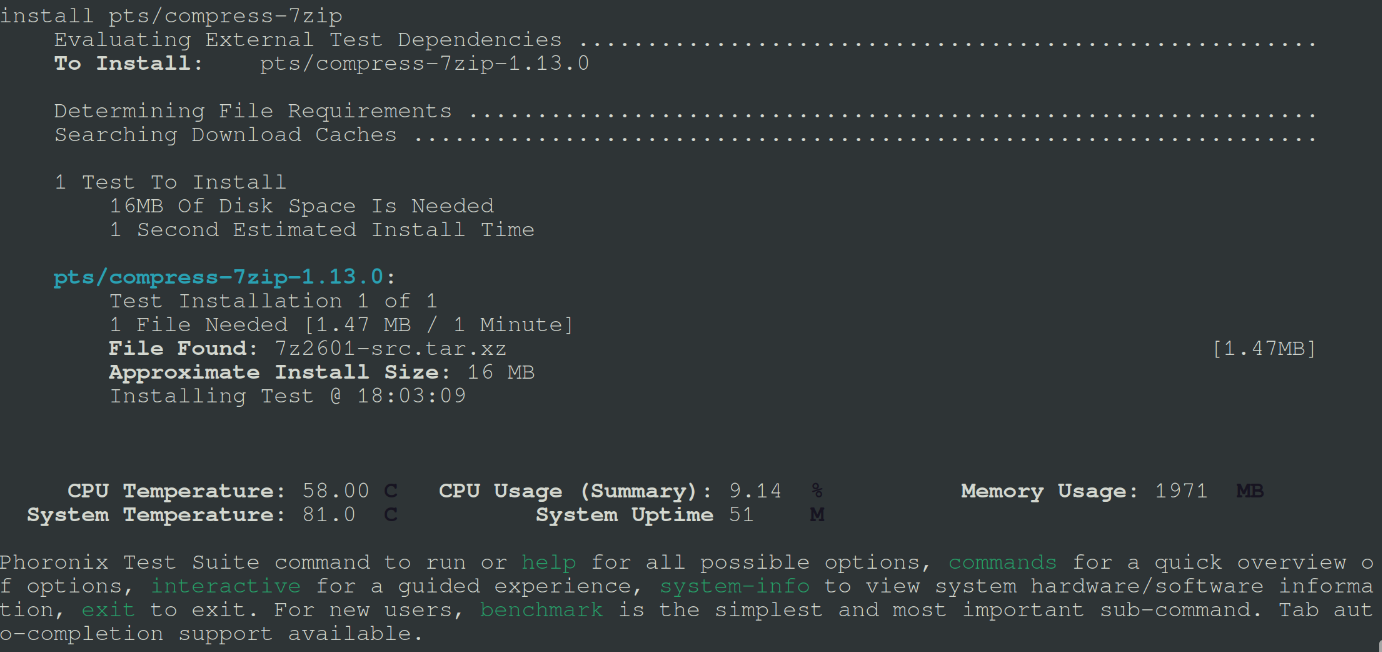
\includegraphics[width=1\textwidth]{../../capturas2/seccion1/instalacion_test.png}

    \caption{Instalación del test a ejecutar. Anteriormente se instalaron las dependencias necesarias.}

\end{figure}
\begin{figure}[H]
    \centering

    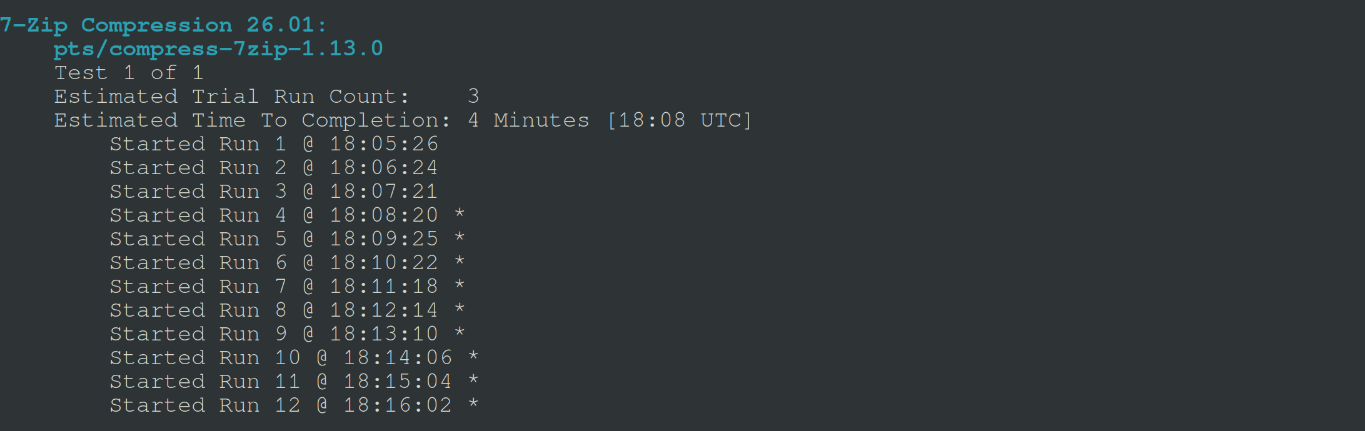
\includegraphics[width=1\textwidth]{../../capturas2/seccion1/ejecucion.png}

    \caption{Ejecución del benchmark.}

\end{figure}
\begin{figure}[H]
    \centering

    
\includegraphics[width=1\textwidth]{../../capturas2/seccion1/guardar_resultados.png}

    \caption{Guardado de los resultados del benchmark.}

\end{figure}
\begin{figure}[H]
    \centering

    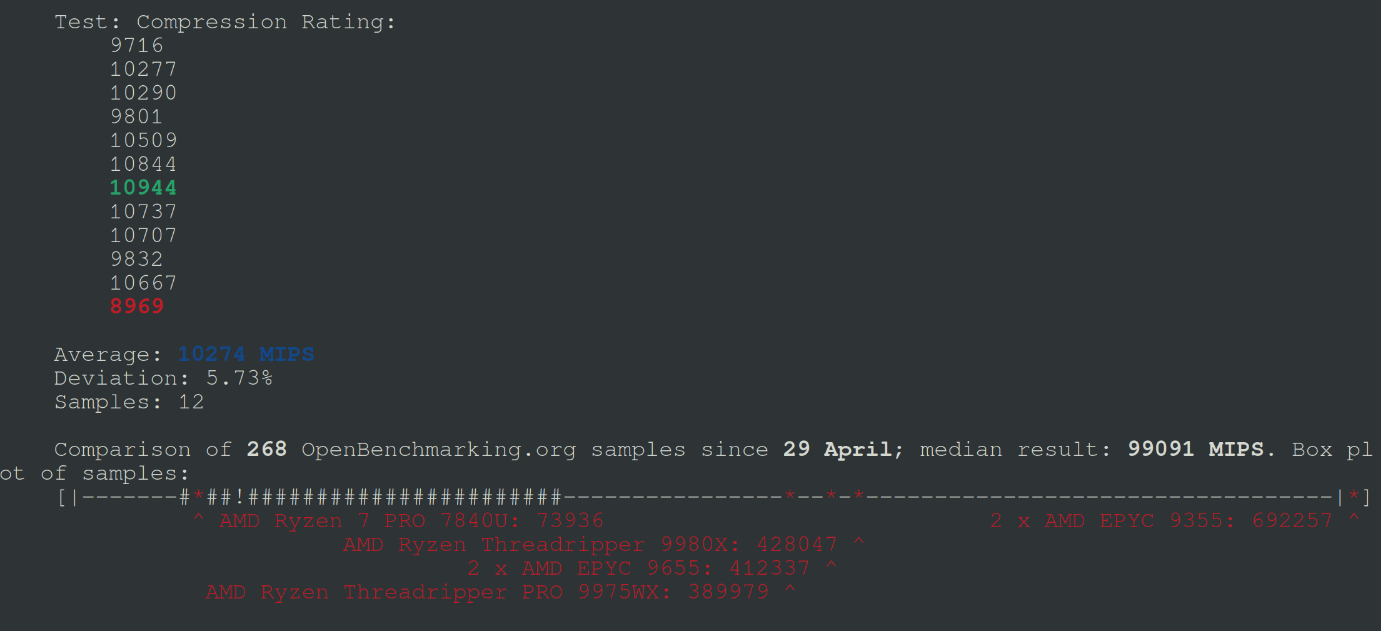
\includegraphics[width=1\textwidth]{../../capturas2/seccion1/comprimir.png}

    \caption{Resultados de compresión.}

\end{figure}
\begin{figure}[H]
    \centering

    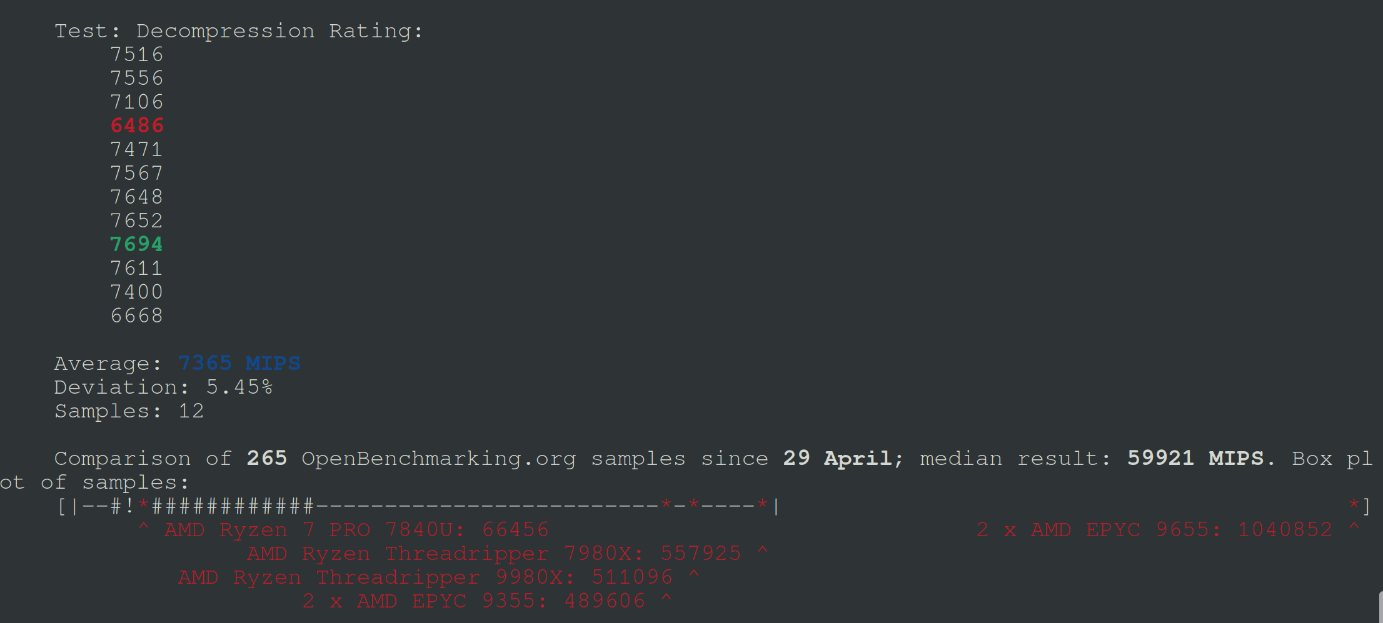
\includegraphics[width=1\textwidth]{../../capturas2/seccion1/descomprimir.png}

    \caption{Resultados de descompresión.}

\end{figure}
\begin{figure}[H]
    \centering

    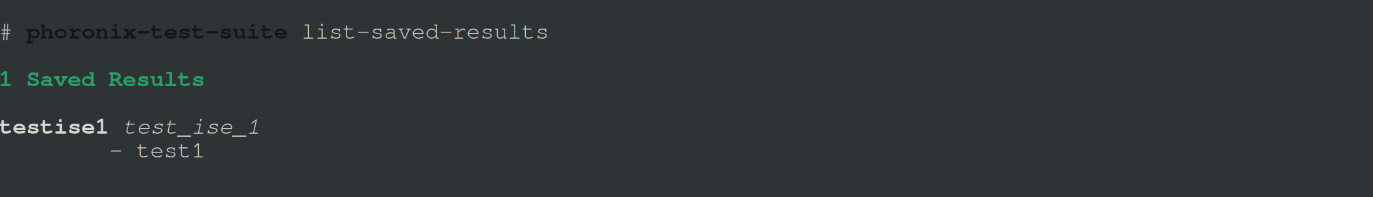
\includegraphics[width=1\textwidth]{../../capturas2/seccion1/ver_guardados.png}

    \caption{Verificación de los resultados guardados.}

\end{figure}
\begin{figure}[H]
    \centering

    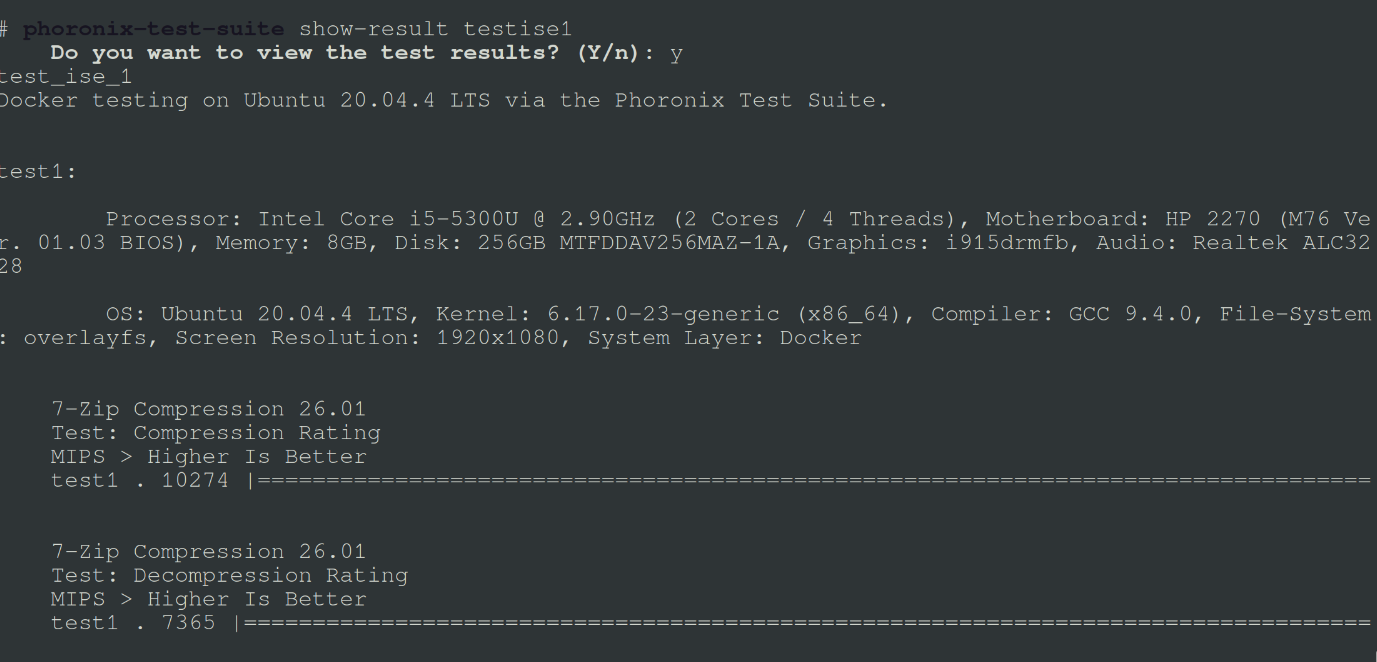
\includegraphics[width=1\textwidth]{../../capturas2/seccion1/mostrar_resultados.png}

    \caption{Mostrando los resultados del benchmark con el comando para ver los test anteriores.}

\end{figure}

El benckmark elegido fue 7-Zip Compression, que evalúa el rendimiento de compresión y descompresión 
de archivos utilizando el algoritmo LZMA.
La elecición de este benchmark se debió a ser un test de procesador según la lista de benchmarks 
recomendados por Phoronix, y por ser un test que se ejecuta en un tiempo razonable.
Podemos ver como el bechmark se ejecuto sin problemas hasta hacer un total de 12 pasadas para evitar 
problemas de variabilidad en los resultados.
\\
Con respecto a los resultados obtenidos, podemos ver una puntuación media de 10.274 MIPS en compresión 
y 7.365 MIPS en descompresión. Esto coloca a nuestro procesador muy abajo con respecto a la mediana de 
Openbenchmarking.org y con respecto a otros procesadores modernos. Muy entendible teniendo en cuenta que 
el procesador del equipo es un Intel Core i5-5300U, un procesador de portátil de hace varios años.

\end{document}